
%template setup, made it adhere to UWA standards
\documentclass[12pt, a4paper]{article}
\usepackage{graphicx}
\usepackage{amsmath}
\usepackage{url}

%fix caption formatting
\usepackage[font=small,labelfont=bf]{caption}

%slightly modified UWA setup
\setlength{\oddsidemargin}{0.5cm}
\setlength{\evensidemargin}{0.5cm}
\setlength{\topmargin}{-1.6cm}
\setlength{\leftmargin}{0.5cm}
\setlength{\rightmargin}{0.5cm}
\setlength{\textheight}{24.00cm} 
\setlength{\textwidth}{15.0cm}
\parindent 0pt
\parskip 5pt
\pagestyle{plain}


%meta info
\title{The RNA Bond Problem}
\author{Max Ward \\
School of Computer Science \& Software Engineering \\
The University of Western Australia}
%let the date get auto generated

%author list formatter. not really needed here, but always nice to have
\newcommand{\namelistlabel}[1]{\mbox{#1}\hfil}
\newenvironment{namelist}[1]{%1
\begin{list}{}
    {
        \let\makelabel\namelistlabel
        \settowidth{\labelwidth}{#1}
        \setlength{\leftmargin}{1.1\labelwidth}
    }
  }{%1
\end{list}}



%-------------------------------------------------------------------------

\begin{document}


%title first!
\maketitle

\begin{abstract}
Ribonucleic Acid (RNA) is an important biological molecule with myriad functions. For example, it drives developmental processes, regulates the expression of genes. Because of this, algorithms for predicting RNA structures have been proposed. The problem they attempt to solve is called the RNA folding problem. In this report, I formally describe a simplified version of this problem, which I call the RNA bond problem. I show that this is equivalent to finding the maximum weight independent set of a circle graph, which is a common problem in VLSI design, bioinformatics, and register allocation for optimizing compilers. I then describe the Nussinov algorithm, which efficiently solves the RNA bond problem. Finally, I compare this algorithm to existing algorithms for solving the maximum weight independent set of a circle graph. It is noteworthy that nobody has yet recognized that these problems are equivalent. This highlights the issues associated with cliquing within scientific communities.
\end{abstract}


{\bf Keywords:} Ribonucleic acid, structure, prediction, empirical, comparison.

{\bf CR Classification:} J.3 Biology and genetics.

\clearpage

%\tableofcontents
%\listoffigures
%\clearpage

\section{Introduction}
Ribonucleic Acid (RNA) performs numerous important biological functions. Some recently discovered and notable examples include its ability to regulate the expression of certain genes \cite{mattick2007new}. It has also been implicated as the driving molecule behind developmental processes \cite{mattick2007new}. Because function is determined by structure, algorithms for predicting the structure of RNA molecules have been under active investigation since the early 1970s. The problem of predicting RNA structure is called the RNA folding problem. I describe a simplified version of this, which I call the RNA bond problem. Furthermore, I introduce the Nussinov algorithm, which solves the RNA bond problem. Finally, I show that the RNA bond problem is equivalent to finding the maximum weight independent set of a circle graph. The implications of this are then discussed.

\section{The RNA Bond Problem}

\begin{figure}
\begin{center}
\scalebox{0.19}{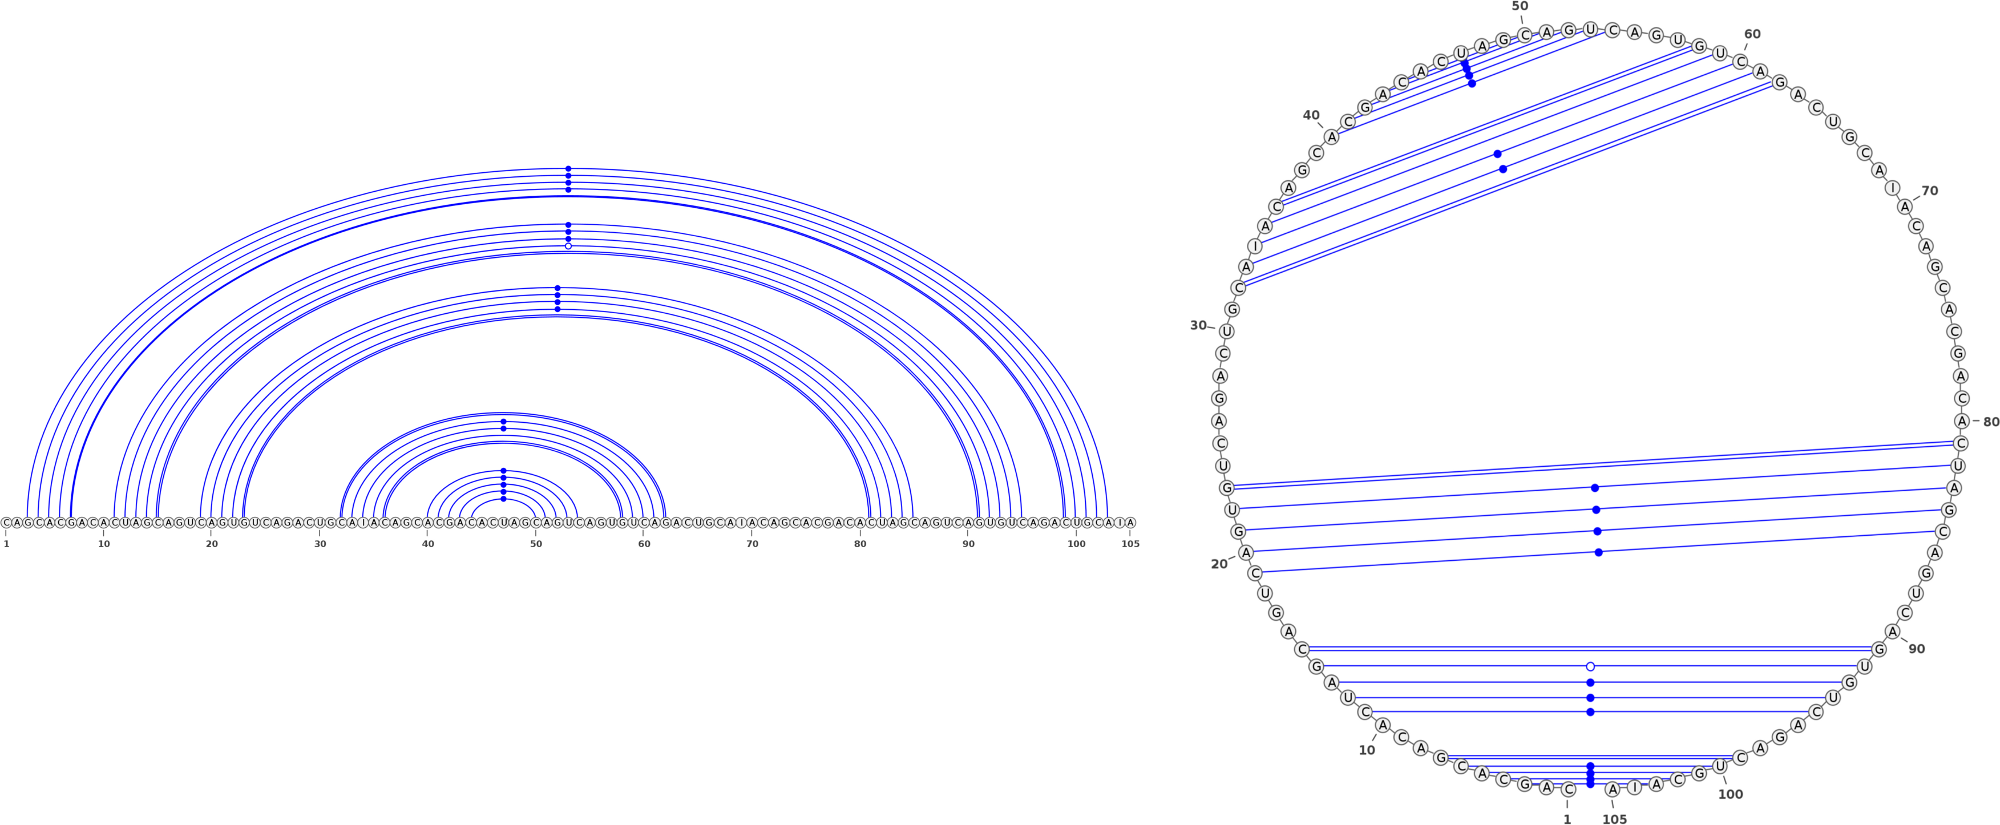
\includegraphics{line2circle}}
\end{center}
\caption{The left diagram is an RNA laid out with its nucleotides in a line. Bonds are represented as blue arcs. In the right diagram, the same RNA, with the same bonds, is represented using a circle diagram.}
\label{fig:line2circle}
\end{figure}

Before the RNA bond problem can be explained, some terminology and background information must be covered. A RNA molecule comprises a sequence of nucleotides connected in sequence. This is often described as a chain. The four RNA nucleotides are Adenosine (A), Uracil (U), Cytosine (C), and Guanine (G). Chemical bonds may form between Adenosine and Uracil; such a bond is called an A-U bond. Other valid bonds are G-U, and G-C. Every bond causes the nucleotide chain to fold on itself. Successive folds lead to the complex, paper-clip like structures common to RNA molecules. For the sake of illustration, let us imagine a RNA nucleotide chain as being connected end to end, thus forming a circle. An example of this is shown visually in Figure \ref{fig:line2circle}. A valid bond is any chord crossing from one nucleotide to  another nucleotide, such that they form a chemically valid bond (A-U, G-C, or G-U). In addition, a valid bond must not cross any other chord in the circle. Finally, every bond has a weight, which indicates the strength of the bond. Given a RNA sequence, the RNA bond problem involves finding a set of valid bonds having maximum weight. In other words, we must find a collection of mutually valid chords such that their sum weight is maximized. I shall now outline an algorithm which solves this problem.

\subsection{The Nussinov Algorithm}
In 1978 Nussinov et al. \cite{nussinov1978algorithms} described an algorithm that can efficiently find solutions to the RNA bond problem. However, this is not by design. The algorithm was originally introduced to solve the RNA folding problem. Nussinov et al.'s intuition was that every bond increases the stability of a RNA's structure, so a structure with maximum bonds should be maximally stable. The Nussinov algorithm is no longer used in practice, as better algorithms now exist for solving the RNA folding problem. I describe it here only because it solves the RNA bond problem.

The nucleotides which make up a RNA sequence can be indexed from zero to $n-1$ where $n$ is the length of the RNA sequence. In addition, let the weight of a bond between nucleotides $i$ and $j$ be defined by $W(i,j)$. Also, the function $M(i,j)$ returns the solution to the RNA bond problem considering only nucleotides between $i$ and $j$ inclusive. This function is defined by the recurrence relation presented below in Equation \ref{eq:nuss_eq}.

\begin{align} \label{eq:nuss_eq}
	M(i, j) &= \max \left\lbrace A, B, C, D \right\rbrace \nonumber  \\
	A &= M(i, j-1) \nonumber \\
	B &= M(i+1, j) \nonumber \\
	C &= M(i+1, j-1) + W(i, j) \nonumber \\
	D &= \max \left\lbrace M(i, k) + M(k+1, j) \right\rbrace \: for \: all \: k \: where \: i < k < j \nonumber	\\
\end{align}

This function can solve the RNA bond problem, $M(0, \ \texttt{RNA\_Length}-1)$. The first two cases ($A$ and $B$) find the score associated with not allowing the bases corresponding to indexes $i$ and $j$ to bond. Case $C$ conversely determines the score given that $i$ and $j$ are bonded. The final case $D$ computes the score associated with a bifurcation. A bifurcation is the decomposition of RNA into two separate structures. This recurrence relation is solved using dynamic programming. As such, it implies a $O(n^3)$
worst case time complexity and a $O(n^2)$ space complexity, as a $O(n^2)$ state space (all combinations of $i$ and $j$) is explored
with a linear time recurrence relation.


\section{Maximum Weight Independent Sets and Circle Graphs}

\begin{figure}
\begin{center}
\scalebox{0.19}{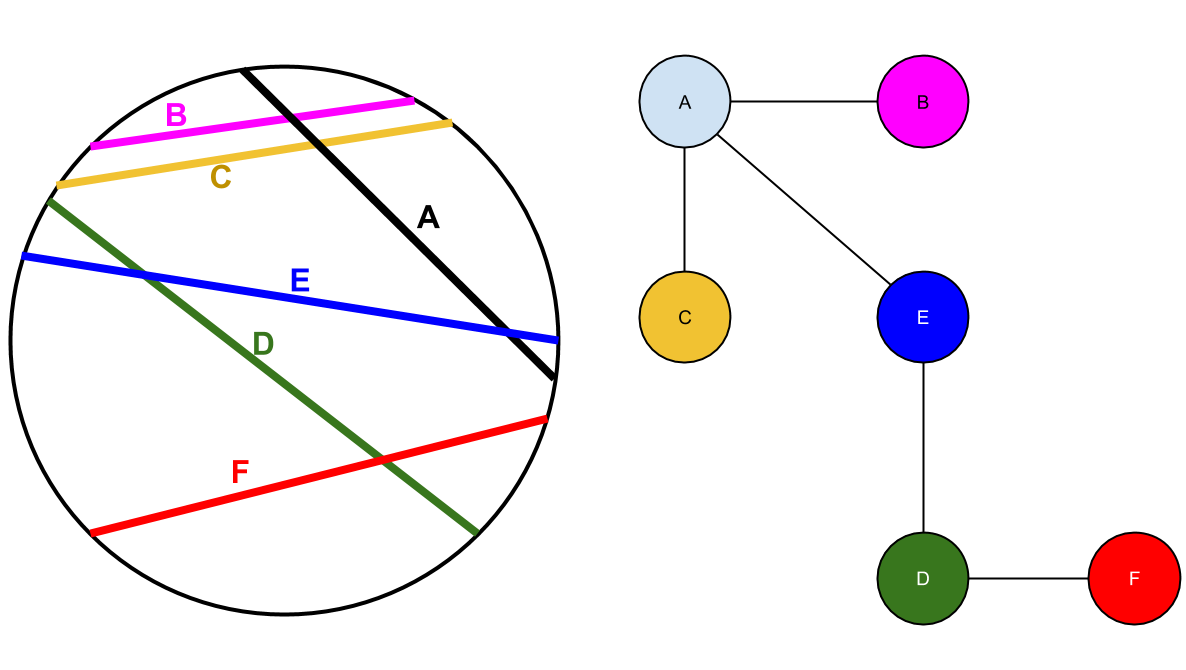
\includegraphics{circle2graph}}
\end{center}
\caption{The left is an example circle diagram. On the right, a circle graph that represents the circle diagram is given. All chords are letter and colour coded.}
\label{fig:circle2graph}
\end{figure}

An independent set of a graph is any collection of vertices such that none share an edge. The maximum weight independent set of a graph requires that vertices have weights. It is defined as any independent set such that the sum weight of vertices is maximal. A circle graph is a special kind of graph derived from a circle diagram. A circle diagram is easy to visualize. Imagine a circle and a collection of chords crossing the inside edge of the circle. This is a circle diagram. A circle graph is derived from a circle diagram using a simple procedure. Every chord is represented by a vertex. Two vertices share an edge if and only if the chords they represent intersect in the circle diagram. This is best explained using a diagram, thus I have included Figure \ref{fig:circle2graph}. Finding the maximum weight independent set of a circle graph is equivalent to finding a set of non-intersecting chords with maximum sum weight in the circle diagram.

Finding the maximum weight independent set of a circle graph has several practically important applications. For example, it is used in register allocation \cite{de1999graph}, VLSI design \cite{cong1990over}, and bioinformatics \cite{swenson2009maximum}.


\subsection{Graphs and RNA}
I wish to point out that the RNA bond problem is isomorphic to finding the maximum weight independent set of a circle graph. This is the core observation of this report. If we imagine a RNA joined end to end in a circle, and all of the possible valid bonds represented as chords across the circle, the solution to the RNA bond problem is any subset of chords that do not intersect, and which has maximum sum weight. This is, by definition, also a maximum weight independent set. As such, the Nussinov algorithm finds the maximum weight independent set of a circle graph.

Borrowing terminology from literature on graph theory, I shall refer to the number of distinct points on a circle graph as $n$, and the number of chords as $m$. In other words, there are $m$ chords, and there are $n$ distinct points where a chord or chords touch the interior edge of the circle diagram. Thus, we say that the Nussinov algorithm takes $O(n^3)$ time. The Nussinov algorithm was published in 1978. The most optimal algorithm for finding the maximum weight independent set of a circle graph at the time required $O(m^3)$ time, and was discovered in 1973 \cite{gavril1973algorithms}. This is inferior to the Nussinov algorithm, as $m$ is bounded from below by $n / 2$. It wasn't until 2003 that a clearly better algorithm was found. This algorithm required $O(md)$ time, and was discovered by Valiente \cite{valiente2003new}. Note that $d$ represents the density of the graph, but the precise complexity analysis is not important for this discussion. Despite the Nussinov algorithm being an asymptotically superior algorithm for 25 years, it was never used outside of RNA research.


\section{Conclusions}
I have briefly introduced the RNA folding problem. Following this, a precise definition of a simpler problem, the RNA bond problem, was described. The Nussinov algorithm is a relatively simple and reasonably efficient solution to this problem. In addition, I have shown that the RNA bond problem, and finding the maximum weight independent set of a circle graph, are equivalent. Thus, the Nussinov algorithm solves both problems. In addition, it was more optimal than the other algorithms that solved the same problem at the time of its publication. This has not been recognized until now. I submit that this illustrates the danger of over specialization within scientific communities. I also conjecture that this situation would have been avoided with a more holistic approach to research. All
knowledge is valuable; insular research has no place in the advancement of science


%let bibtex do all the hard work
\bibliographystyle{plain}
\bibliography{assignment_one}


\end{document}

